\documentclass[uplatex]{jsarticle}
\usepackage[utf8]{inputenc}

\usepackage{amsmath}
\usepackage[dvipdfmx]{graphicx}
\usepackage{resume}  % resume用スタイル
\usepackage{udline}  % 下線用
\usepackage{comment} % 複数行コメント
\pagestyle{plain}
 
\begin{document}
\twocolumn[
    \beginheader{令和5年度 コンピュータサイエンス学部 中間発表}{2023}{8}{9}{井上 研究室}
    \title{VR環境での落下感に姿勢が与える影響}
    \author{C0B20205 武田 夢音 (Yumene Takeda)}
    \endheader
]
\vspace{3mm}

%%ページ番号
\setcounter{page}{9}

\section{はじめに}
シミュレーション中に体の角度を変えながら落下を体験することができるデバイスの利点を書く

\begin{figure}[tb]
  % width や height で絶対的な大きさ指定をすることもできる
  \centering
  \fbox{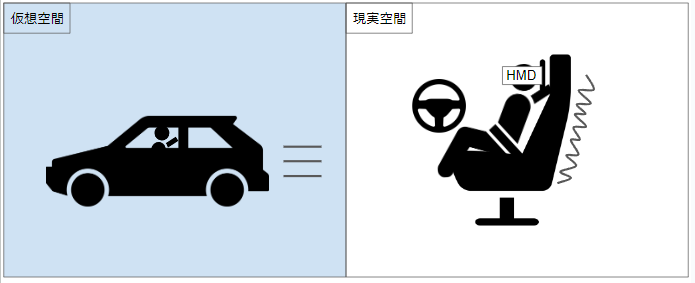
\includegraphics[width=1\linewidth]{fig/about_system.png}}
  \caption{システム概要図}
  \label{fig:about_system}
  \fbox{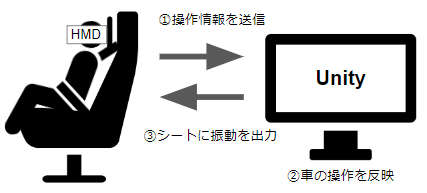
\includegraphics[width=1\linewidth]{fig/system_str.png}}
  \caption{システム構成図}
  \label{fig:system_str}
\end{figure}

\section{関連研究}
王らの研究はドライビングシミュレータであるアクセスマスターAM2330を使用して行われた.このシミュレータには自動車の加減速に応じた座席の振動と,車体振動を模擬した振動を付加する機能があり,これを用いて自動車の運転経験豊富なプロドライバー6名を被験者にして実験を行った.

齋藤らは後頭部と臀部への振動がVR酔いに対してどう影響するかを検証した\cite{cybsick_delay_by_vibrate}
.
後頭部に振動装置を追加したHMDと座面に振動装置を追加したクッションを制作し,それぞれの部位に振動を与えた場合と与えない場合で実験を行うことで後頭部への振動がVR酔いの発生を遅延させることが明らかにされた.


\section{VR振動提示システム}
\subsection{システム概要}
システム概要を\figref{fig:about_system}に示す.現実空間にはシートやハンドル,アクセルとブレーキなど実際の車と同じ環境を用意し,VRヘッドセットを装着させる.

仮想空間には自動車オブジェクトを用意し,VRヘッドセットの視点はその自動車の運転席に固定する.現実空間での操作に応じて仮想空間内の自動車が動作し,自動車の加減速によってシートに振動が与えられる.

また,加減速によって与えられる振動とは別に,エンジンの振動を模した振動をシートに常時与える.

\subsection{システム構成}
システム構成を\figref{fig:system_str}に示す.本システムはHMD,アクセルやブレーキなどの運転機器,振動装置を取り付けたシートから構成される.ユーザはHMDを通して仮想空間を見ており,運転機器の操作状態をコンピュータに送信する.コンピュータではそれらの情報を元に仮想空間内の自動車を操作し,操作に応じた振動をシートに与える.

仮想空間を実装するソフトウェアはUnityを想定している.




\section{評価方法}
先行研究では評価にSchefféの一対比較法を用いて運転時に感じる「現実感」,「走行感」,「快適さ」を計測していたため,本研究でも同様の評価方法を用いる.

ここで用いる「現実感」とは実際に自動車に乗っているような感覚,「走行感」とは自動車で走って前へ進んでいるような感覚,「快適さ」とはVR環境のドライビングシミュレータで運転している時の心地よさ・気持ち悪くなさのことと定義した.

振動を付加した場合としなかった場合の2種類の条件下で1回の運転時間が約3分となるコースを走行させる.

その後,その2条件について実験参加者に評価を求める.

\section{検討事項}
本研究の検討事項は3つある.
1つ目は仮想空間内の自動車の種類である.普通自動車や2輪車,大型トラックなど自動車には種類があるが,現在想定しているのは普通自動車だけであり,他の種類の自動車に対しての実験が必要であるかについて検討が必要である.

2つ目は被験者についてである.先行研究では運転経験の豊富なプロドライバーを被験者としていたが,そのような被験者を集めることは難しいため,被験者は多少の運転経験があるアマチュア程度になると考えられる.
しかし,先行研究では運転経験の豊富な人ほどシミュレータ酔いを起こしやすいという理由でプロドライバーを被験者として選択しているため,被験者がアマチュアの場合に正確な結果を得ることが出来るかどうかは検討が必要である.

3つ目は振動の詳細についてである.先行研究では振動の強弱や種類・位置について細かく記載されていないため,それらについても検討する必要がある.特に振動位置については齋藤らの研究によって振動を与える体の部位によって効果が異なることが示されたため,検討が必要である.

\section{まとめ}
本研究ではVR環境での運転シミュレーション酔いに振動が与える影響についての調査を行う.今後はシステム実装と実験を行い,課題を解決できたかを評価する.


 \bibliographystyle{junsrt}
\bibliography{ref.bib}   % 参考文献のデータベースファイルを指定する 
\end{document}
